\documentclass[a4paper, 12pt]{article}
\usepackage[T2A,T1]{fontenc}
\usepackage[utf8]{inputenc}
\usepackage[english, russian]{babel}
\usepackage{graphicx}
\usepackage[hcentering, bindingoffset = 10mm, right = 15 mm, left = 15 mm, top=20mm, bottom = 20 mm]{geometry}
\usepackage{multirow}
\usepackage{lipsum}
\usepackage{amsmath, amstext}
\usepackage{siunitx}
%\usepackage{subcaption}
\usepackage{wrapfig}
\usepackage{mathrsfs}
\usepackage{adjustbox}
\usepackage{enumerate, indentfirst, float}
\usepackage{pgffor}
\usepackage{capt-of, svg}
\usepackage{array}
\usepackage{longtable}
\usepackage{csvsimple}
\usepackage{pdfpages}
\usepackage{subfigure}
\usepackage{sectsty}

\newenvironment{bottompar}{\par\vspace*{\fill}}{\clearpage}
 
\sectionfont{\fontsize{12}{18}\selectfont}

\begin{document}
\begin{titlepage}

\newcommand{\HRule}{\rule{\linewidth}{0.5mm}} % Defines a new command for the horizontal lines, change thickness here

\center % Center everything on the page
 
%----------------------------------------------------------------------------------------
%	HEADING SECTIONS
%----------------------------------------------------------------------------------------

\textbf{\LARGE Московский Физико-Технический}
\\[5pt]
\textbf{\LARGE Институт}\\[1,5cm] % Name of your university/college
\textsc{\Large кафедра общей физики}\\[0.5cm] % Major heading such as course name
\textsc{\large Лабораторная работа  4.2.3}\\[0.9cm] % Minor heading such as course title

%----------------------------------------------------------------------------------------
%	TITLE SECTION
%----------------------------------------------------------------------------------------



{ \huge \bfseries Интерферометр Релея}
\\[1.7cm] % Title of your document




 
%----------------------------------------------------------------------------------------
%	AUTHOR SECTION
%----------------------------------------------------------------------------------------

\begin{minipage}{0.3\textwidth}
	\begin{flushleft} \large
		\emph{Студент:}\\
		\textbf{Илья  Зыков}% Your name
	\end{flushleft}
\end{minipage}
~
\begin{minipage}{0.5\textwidth}
	\begin{flushright} \large
		\emph{Преподаватель:} \\
		\textbf{Вячеслав Петрович Кириллов} % Supervisor's Name
	\end{flushright}
\end{minipage}

\begin{bottompar}
	
	{\large \today}

\end{bottompar}
\vfill % Fill the rest of the page with whitespace

\end{titlepage}

\section*{Цель работы:}

\noindent Ознакомление с интерференцией на двух щелях, устройством и принципом действия интерферометра Релея и с его применением для измерения показателей преломления газов.

\section*{В работе используются: }
\begin{itemize}
\item технический интерферометр ИТР-1; 
\item светофильтр; 
\item баллон с углекислым газом; 
\item сильфон;
\item манометр;
\item краны.
\end{itemize}	

\section{Рабочие формулы}  




\noindent Число полос m между центрами системи полос:
\begin{equation}
\delta n = \frac{\Delta}{l}=m \frac{\lambda}{l}
\end{equation}


\noindent Показатель преломления n исследуемого газа определяется путём сравнения с воздухом при атмосферном давлении:
\begin{equation}
n = n_{\text{возд}}+\delta n
\end{equation}


\noindent Разности показателей преломления газа от разности давлений газа:
\begin{equation}
\delta n = \frac{\alpha}{2k_BT}\delta P
\end{equation}


\section{Оптическая схема}

\begin{figure}[H]
	\centering
	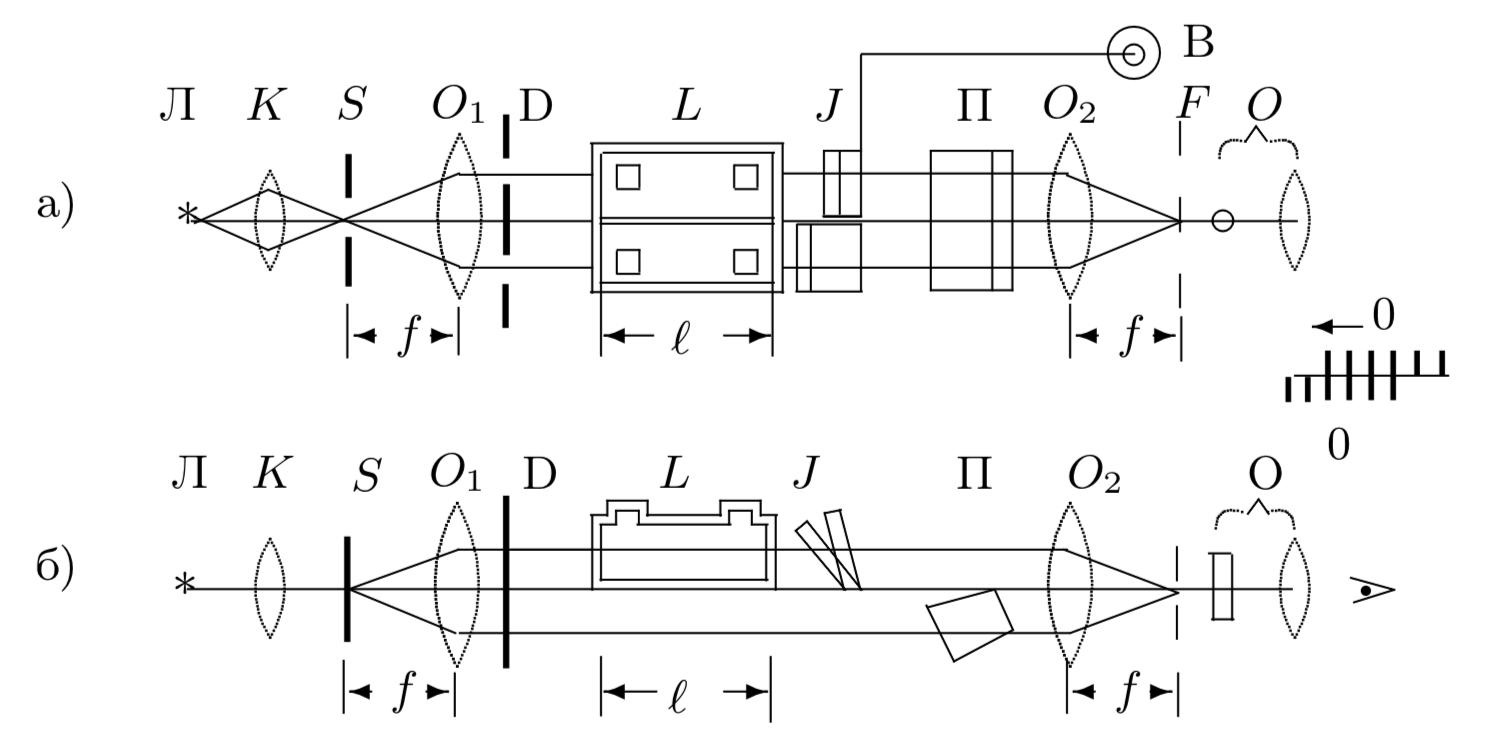
\includegraphics[width = 17 cm]{1.png}
	\caption{Устройство интерферометра Релея: a) вид сверху; б) вид сбоку}
\end{figure}
\[T = 25.01 ^oC\]
\[P = 752.56 \; mmHg\]
\[\lambda = 670\pm50\; nm\]
\[l = 10\; cm\]


\section{Ход работы}
\begin{enumerate}
	\item Прокалибруйте компенсатор в единицах $\lambda$, выделив узкий интервал длин волн с помощью светофильтра
	\item Изменяя давление с помощью сильфона и совмещая нулевые полосы, снимите зависимость показаний компенсатора z от перепада давлений $\delta P$
	\item Заполните углекислым газом камеру с открытым концом. Снимите зависимость равновесного положения компенсатора от времени, раз в минуту совмещая нулевые полосы, и оцените время установления равновесия.

\end{enumerate}
\newpage

\section{Измерения}
\subsubsection*{Калибровка}
\begin{table}[H]
	\centering
	\begin{tabular}{|c|c|c|c|c|c|c|c|c|c|c|c|c|c|}
		\hline	
		
m&-9&-8&-7&-6&-5&-4&-3&-2&-1&0&1&2&3\\ \hline
$z^{calib}$, mm&0.15&0.51&0.87&1.20&1.47&1.80&2.07&2.40&2.75&3.05&3.40&3.63&4.03\\ \hline
m&4&5&6&7&8&9&10&11&12&13&14&15&16\\ \hline
$z^{calib}$, mm&4.34&4.65&4.96&5.33&5.63&5.96&6.21&6.64&6.95&7.29&7.60&7.96&8.14\\ \hline


	\end{tabular}	
	\caption{Полученные значения: калибровка}
\end{table}



\begin{figure}[H]
	\centering
	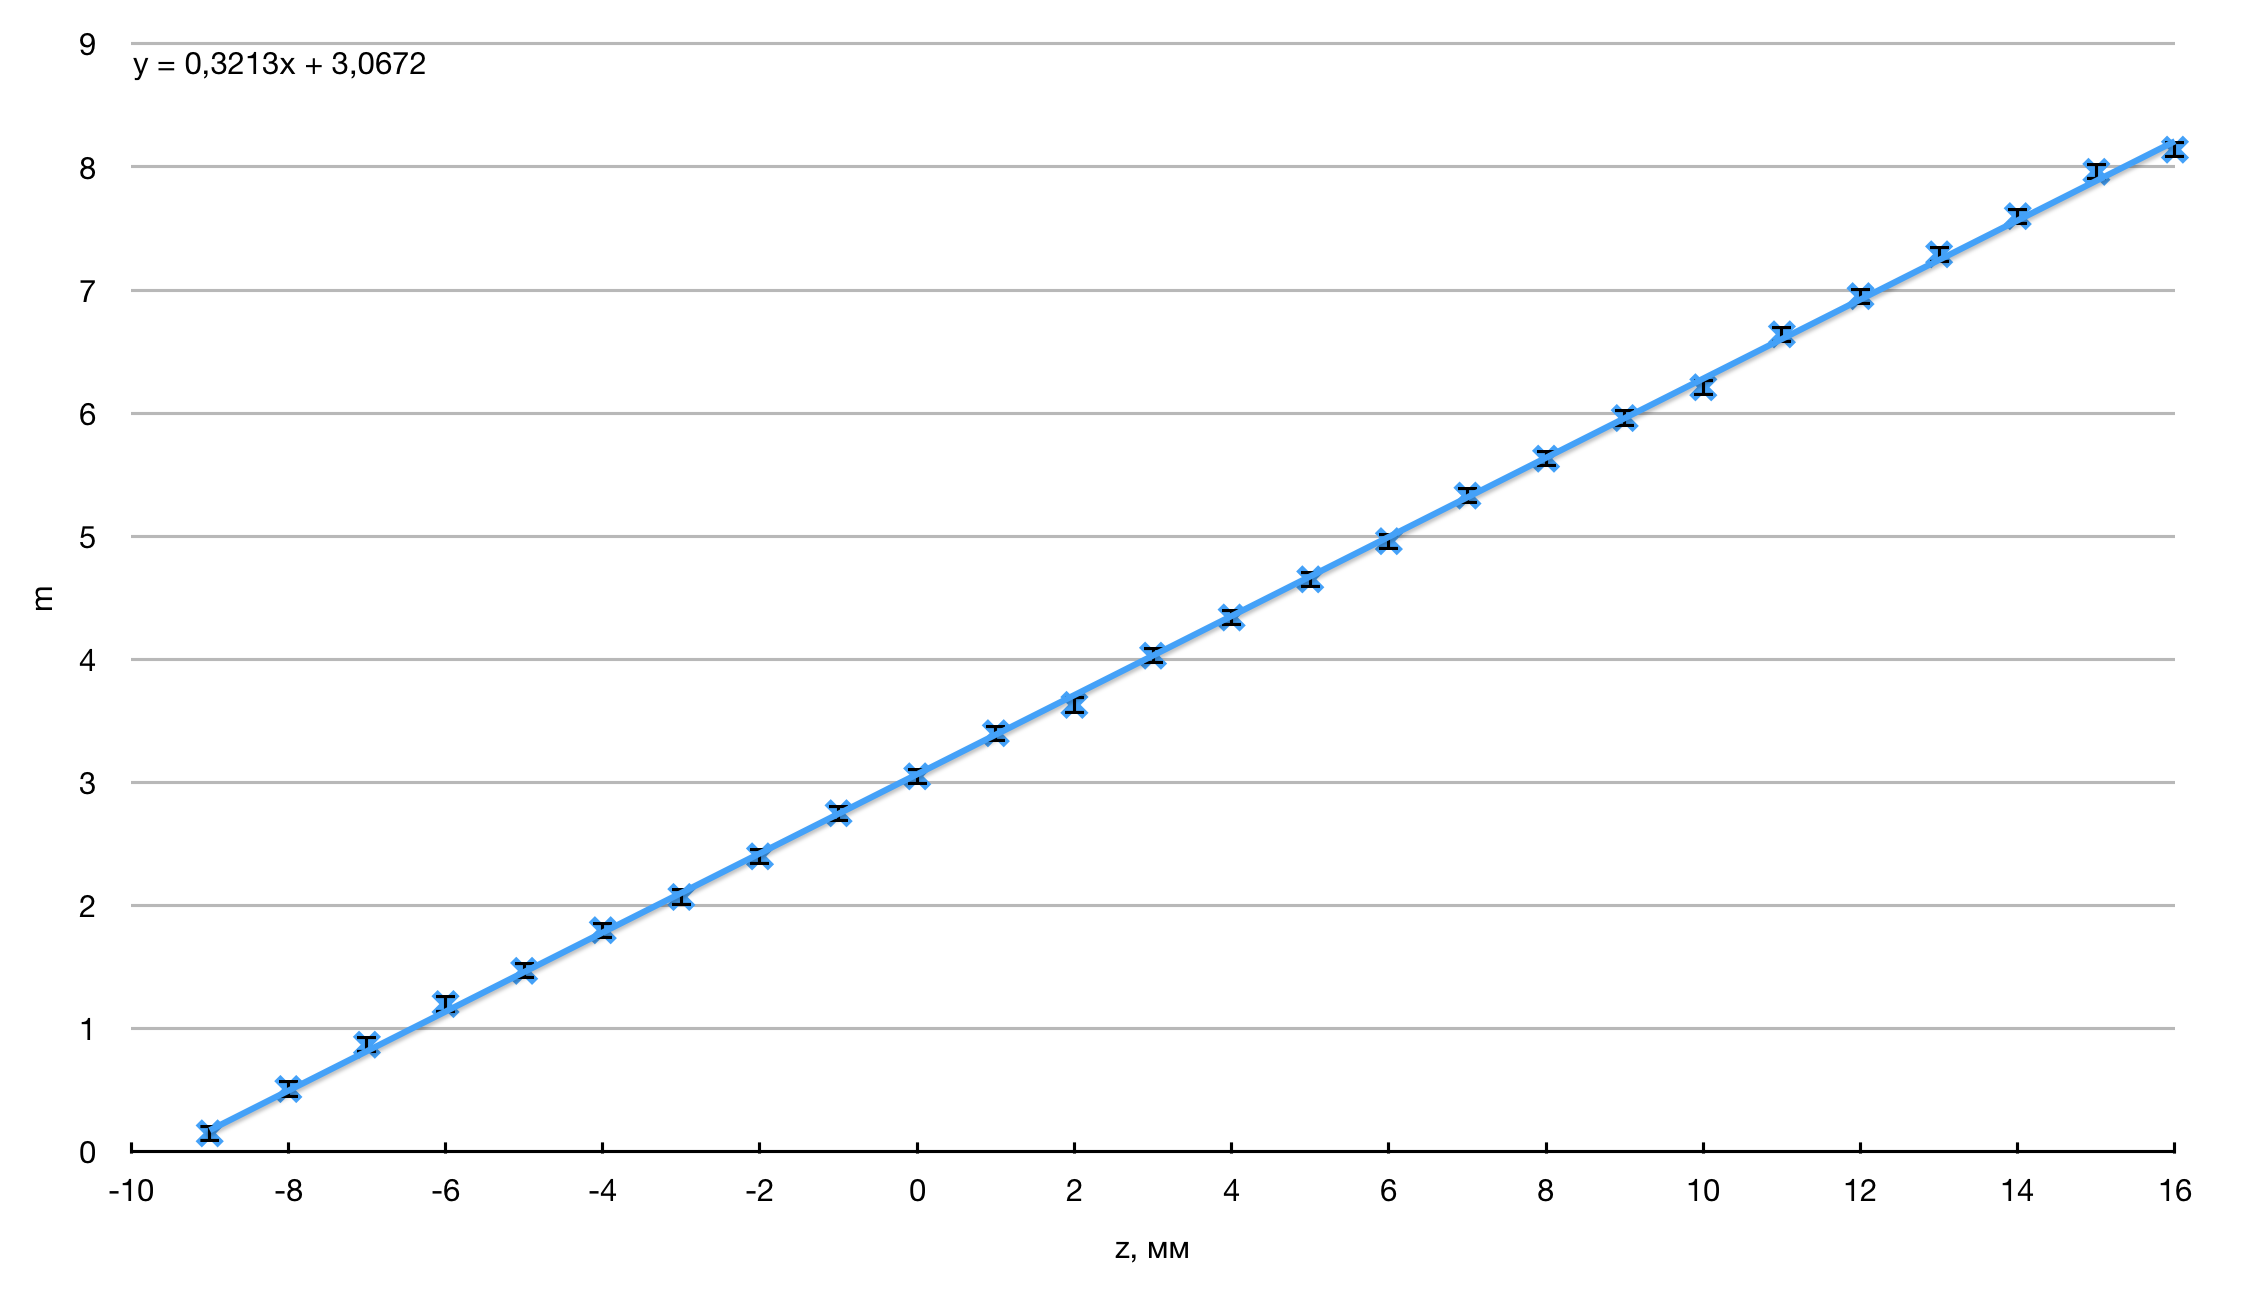
\includegraphics[width = 16 cm]{2.png}
	\caption{Калибровочный график}
\end{figure}

\[m = (0.032\pm0.001)mm^{-1}\cdot z+(3.07\pm0.07)\]
\newpage

\subsubsection*{Зависимости показателя преломления от разности давлений}

\begin{table}[H]
	\centering
	\begin{tabular}{|c|c|c|c|c|c|c|c|c|c|c|c|}
		\hline	
		
	$z^{press}$, mm&3&3.25&3.33&3.47&3.61&3.75&3.85&4.03&4.14&4.24&4.41\\ \hline
	$\delta n, 10^{-6}$&0.000&0.538&0.710&1.011&1.312&1.613&1.828&2.215&2.452&2.667&3.032\\ \hline
	$\Delta P$, мм вод ст&0&-100&-200&-300&-400&-500&-600&-700&-800&-900&-1000\\ \hline
	$z^{press}$, mm&2.99&2.87&2.71&2.63&2.44&2.32&2.17&2.03&1.81&1.72&\\ \hline
	$\delta n, 10^{-6}$&-0.022&-0.280&-0.624&-0.796&-1.204&-1.462&-1.785&-2.086&-2.559&-2.753&\\ \hline
	$\Delta P$, мм вод ст&0&100&200&300&400&500&600&700&800&900&\\ \hline
		
	\end{tabular}	
	\caption{Полученные значения: зависимости показателя преломления от разности давлений}
\end{table}

\begin{figure}[H]
	\centering
	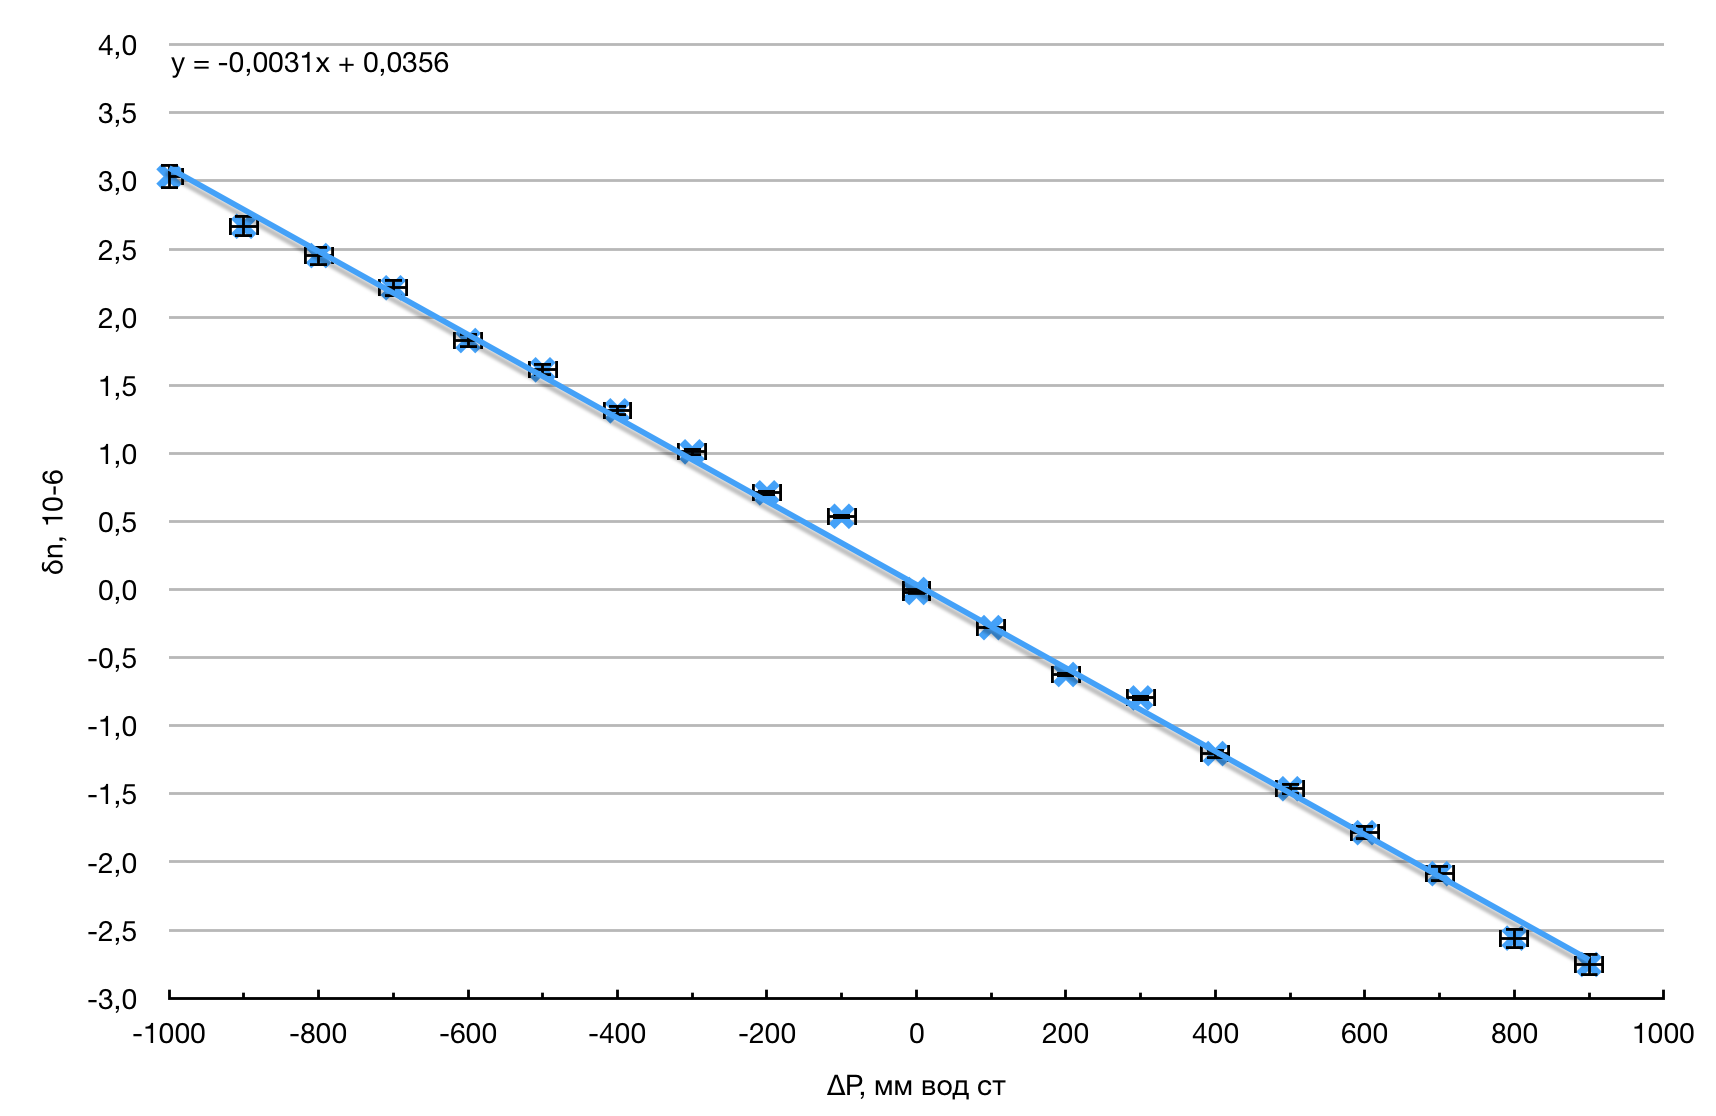
\includegraphics[width = 16 cm]{3.png}
	\caption{График зависимости показателя преломления от разности давлений}
\end{figure}

\noindent Коэфициент угловогог наклона:
\[\kappa = \frac{\delta n}{\delta P} = \frac{\alpha}{2k_BT} \]
\[\kappa = (3.1\pm0.1)\cdot10^{-9} \text{Па}^{-1}\]
\noindent Поляризуемость молекул воздуха:
\[\alpha = 2k_BT\cdot\kappa\]
\[\alpha = (2.55)\cdot10^{-29}m^3\]
\[n=1+\frac{\alpha}{2k_{B}T}P = 1.00031 \]
\noindent Теоретическое значение:
\[n^{theor}=1.00027\]

\newpage
\subsubsection*{Зависимости показателя $CO_2$ от времени}

\begin{table}[H]
	\centering
	\begin{tabular}{|c|c|c|c|c|c|c|c|c|c|c|}
		\hline	
		
	t, min&0&1&2&3&4&5&6&7&8&9\\ \hline
	$z^{time}$, mm&10.04&9.27&7.60&6.71&6.38&6.07&5.78&5.62&5.38&5.29\\ \hline
	$n(CO_2)$&1.00063&1.00060&1.00055&1.00052&1.00051&1.00050&1.00049&1.00049&1.00048&1.00048\\ \hline
	t, min&10&11&12&13&14&15&16&17&18&19\\ \hline
	$z^{time}$, mm&5.17&5.07&4.98&4.95&4.87&4.82&4.81&4.74&4.72&4.70\\ \hline
	$n(CO_2)$&1.00047&1.00047&1.00047&1.00047&1.00046&1.00046&1.00046&1.00046&1.00046&1.00046\\ \hline
	
		
	\end{tabular}	
	\caption{Полученные значения: показатель преломления смеси CO2 с воздухом  от времени}
\end{table}

\begin{figure}[H]
	\centering
	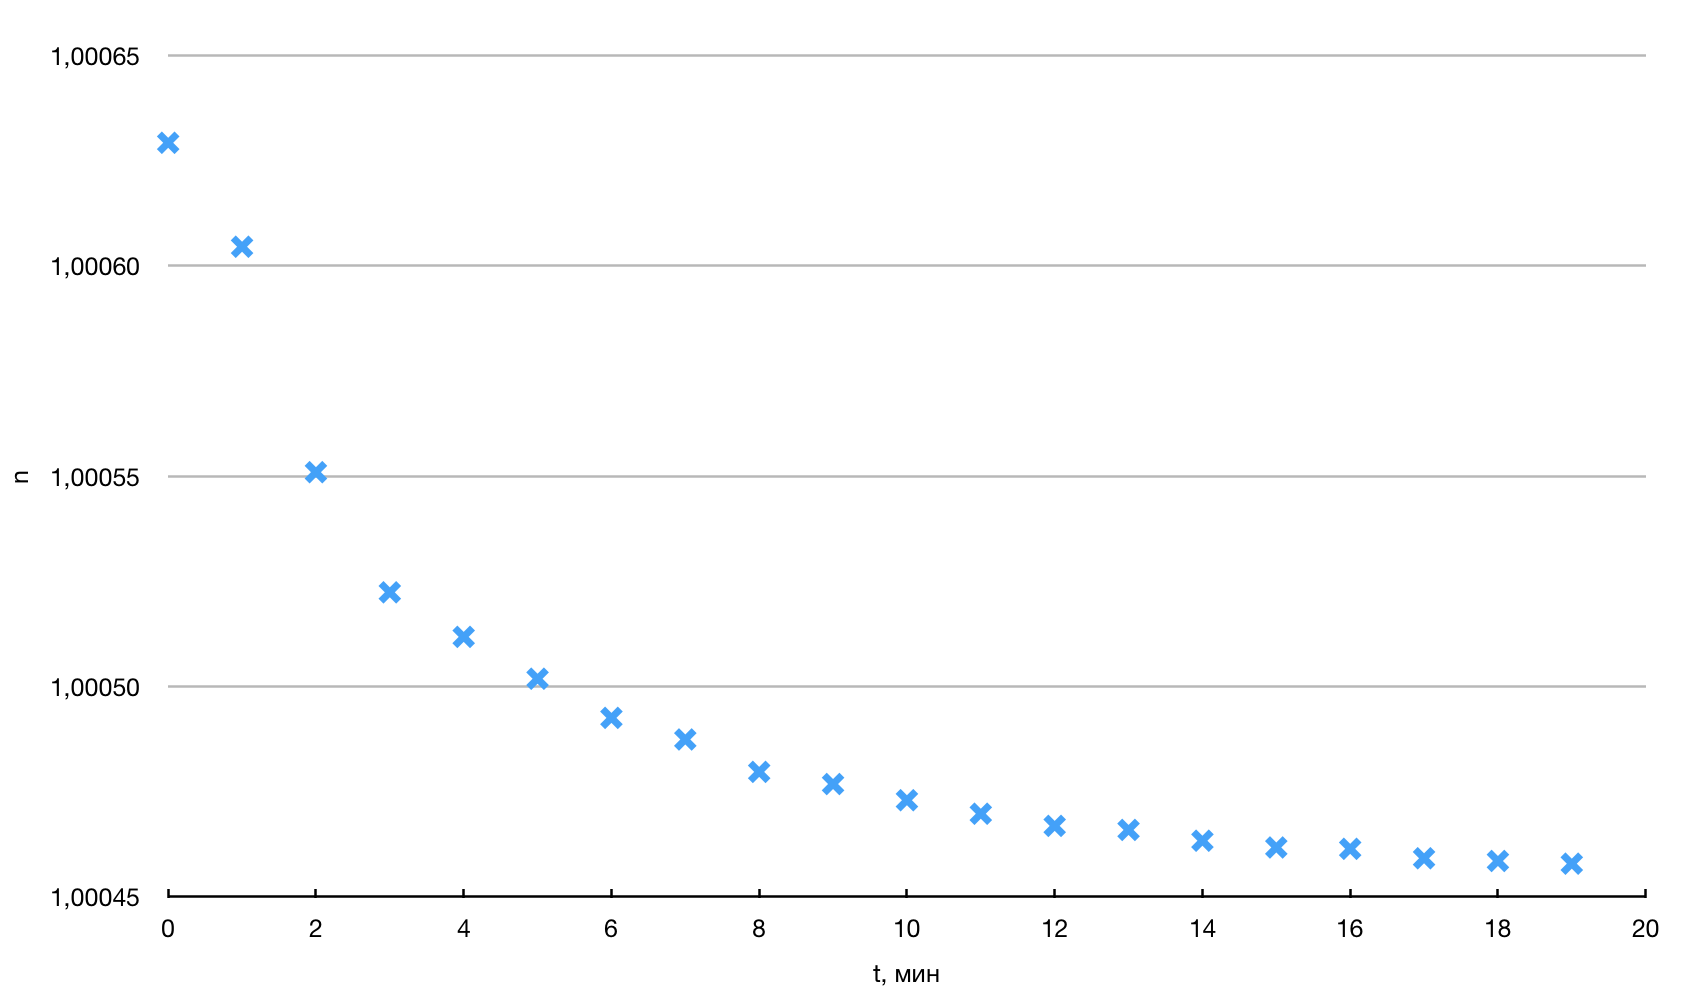
\includegraphics[width = 16 cm]{4.png}
	\caption{График зависимости показателя преломления от времени}
\end{figure}

\[n(CO_2) = 1.00065\pm0.00005\]
\[n^{\text{н.у.}}(CO_2) = 1.00058\pm0.00005\]
\[n^{\text{theor}}(CO_2) = 1.00045\]
\\
\noindent Интервал $\delta n$, возможных для измерения с помощью интерферометра:
\[\delta n = [0.2\cdot 10^{-6} - 16 \cdot 10^{-6}] \]


\section*{Вывод}  
	\noindent В данной работе мы исследовали изменение показателя преломления воздуха при изменении давления и определили разность показателей преломления воздуха и углекислоты при атмосферном давлении. По результатам измерений рассчитывали показатели преломления воздуха и углекислого газа при нормальных условиях, а также диапозон применимости интерферометра. 
\end{document}
